\graphicspath{ {04-KL/Figures/} }

\section{KLOE-Light Calorimeter}
\label{Sect:KL}

The KLOE-Light (KL) pre-shower sampling calorimeter was composed of
extruded lead foils in which scintillating fibres were placed.
At normal incidence the thickness of the detector was 2.5 radiation
lengths.
The detector provided energy deposition and timing information and was
used to distinguish muons from decay
electrons~\cite{2016JInst..11P3001A}.
The KL consisted of a series of layers of 1\,mm diameter BICRON BCF-12
scintillating fibres embedded in an appropriately shaped lead sheets
(see figure~\ref{fig:KL2}).
Each fibre was separated by 1.35\,mm from its neighbours within a
layer and the distance between the centres of the fibres in adjacent
layers was 0.98\,mm.
One layer was shifted by half the fibre pitch with respect to the next.
The volume ratio of scintillator to lead was approximately 2:1,
``lighter'' than the ratio of 1:1 used in the similar calorimeter of the KLOE
experiment~\cite{Ambrosino:2009zza}. 
Lead/scintillator layers were stacked into slabs, 132\,mm in depth.
A total of 7 slabs formed the whole detector, which had an active
volume of 93\,cm$\times$93\,cm$\times$4\,cm.
Scintillation light was guided from each slab into a total of six PMTs
(three at each end).
Iron shields were fitted to each photomultiplier to mitigate the effect of stray magnetic fields.
The signal from each PMT was sent to a shaping amplifier module
that stretched the signal in time to match the sampling rate
of the CAEN 1724 FADCs. \\
\begin{figure}
  \begin{center}
    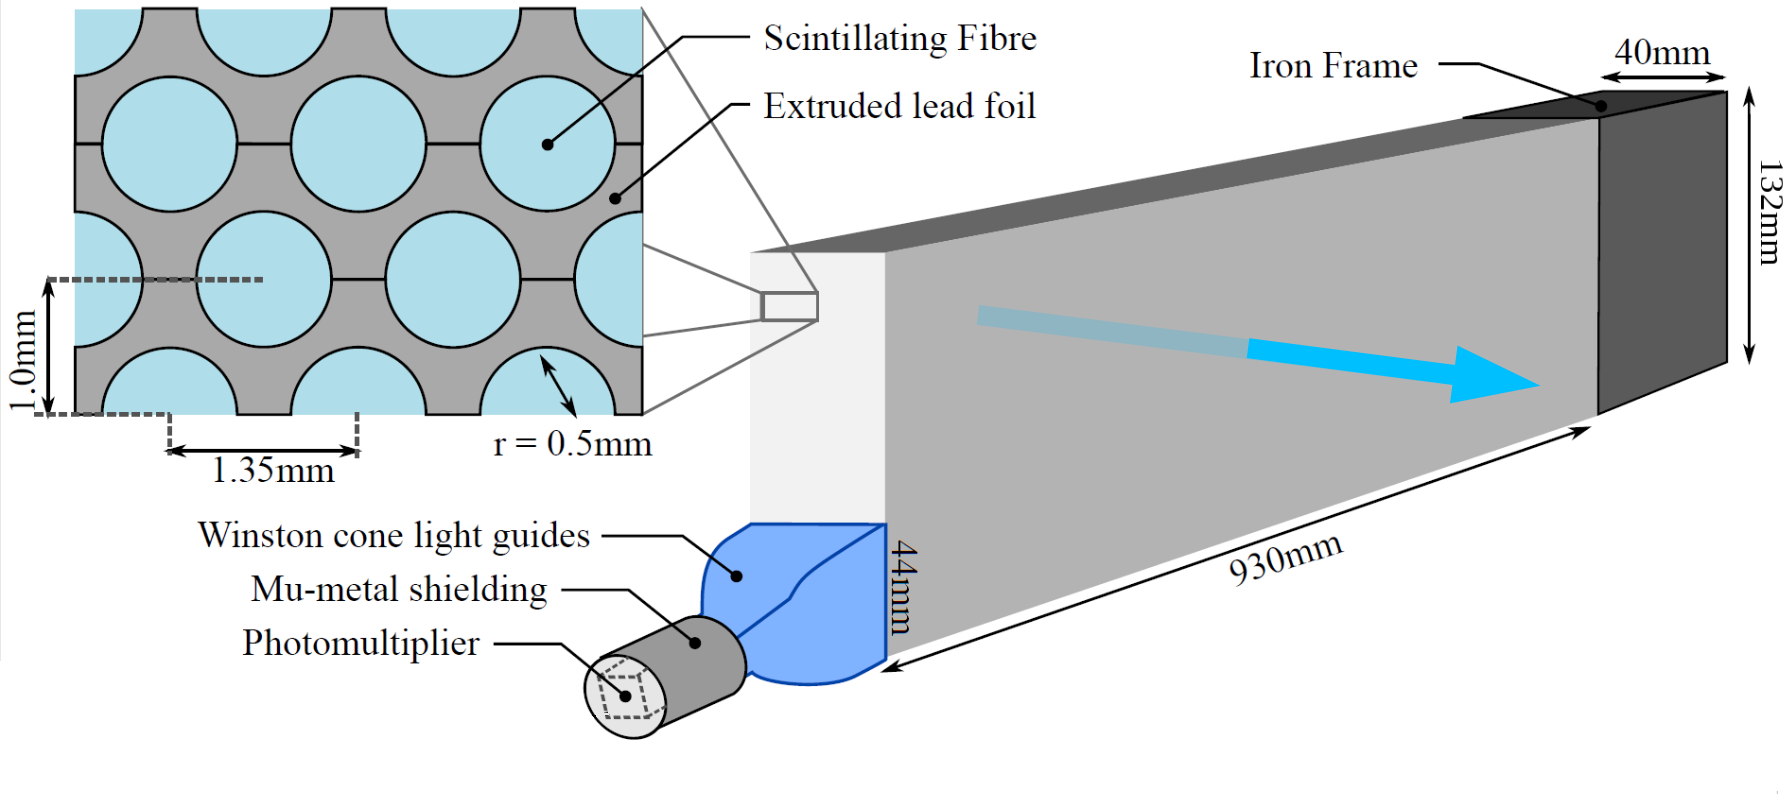
\includegraphics[width=0.85\columnwidth]{./04-KL/Figures/KL2_with_beam.png}
    \caption{Single slab design of MICE KLOE-Light Calorimeter~\cite{Overton:2014tka}; only one of the six PMT assemblies is shown.
    The beam direction is represented by the blue arrow traversing the slab.
    }
    \label{fig:KL2}
  \end{center}
\end{figure}

\noindent\textbf{Performance} \\
\noindent
%The response of the KL to muons, pions, and electrons is shown for various beam momentum settings in~figure~\ref{fig:KL3}.
To study the response of the KL, the particle momentum was determined from the
measured time-of-flight between TOF0 and TOF1.
To compensate for the effect of attenuation the performance was
evaluated in terms of the ``ADC product'' given by:
\begin{equation}
  \text{ADC}_{\text{prod}} = \frac{2 \times
    \text{ADC}_{\text{left}} \times \text{ADC}_{\text{right}}}{
    (\text{ADC}_{\text{left}} + \text{ADC}_{\text{right}})}\,;
\end{equation}
where ADC$_{\text{left}}$ and ADC$_{\text{right}}$ are the signals
from the two ends of a slab and the factor of 2 is present for
normalisation.
Data was taken with no field in the spectrometer solenoids or the
focus coil at beam-momentum settings chosen to span the range of
momenta used during MICE running.
The resulting momentum distributions were centred at 140, 170,
200, 240, and 300\,MeV/$c$.
The response of the KL to muons and pions was observed to increase with
beam momentum.
%\begin{figure}
%  \begin{center}
%    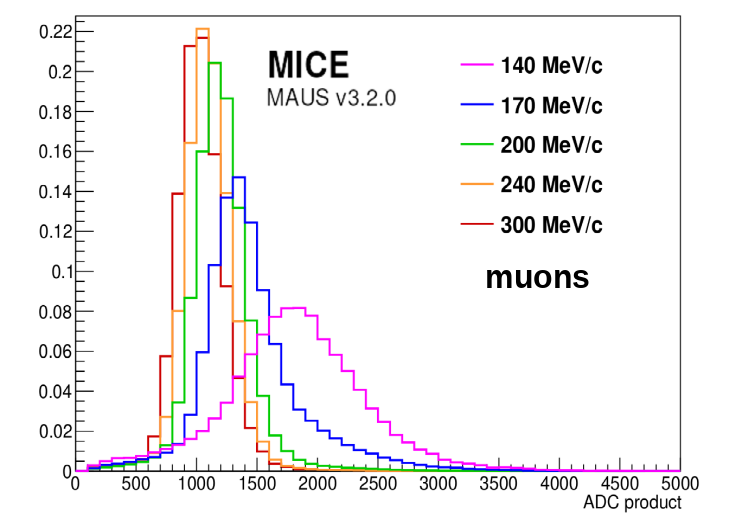
\includegraphics[width=0.45\columnwidth]{./04-KL/Figures/muon-edited.png}
%    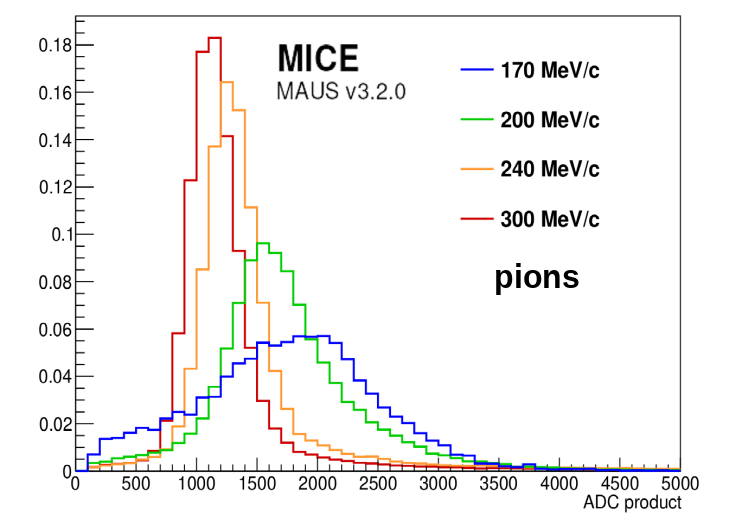
\includegraphics[width=0.45\columnwidth]{./04-KL/Figures/pion-edited.png}
%    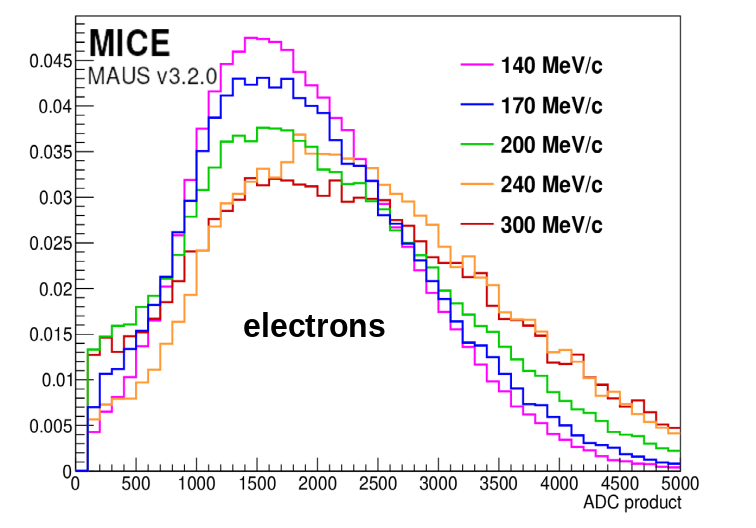
\includegraphics[width=0.45\columnwidth]{./04-KL/Figures/electron-edited.png}
%  \end{center}
%  \caption{
%    KL response to muons (top left), pions (top right) and electrons
%    (bottom) for all available momenta.
%    The charge deposited by particles in KL in arbitrary units is
%    shown.
%    140\,MeV/$c$ pions are irrelevant at the KL position.
%    All histograms are normalised to unity.
%  }
%  \label{fig:KL3}
%\end{figure}
  
Figure~\ref{fig:KL4} presents a comparison of the response to muons,
pions and electrons for various beam momentum settings.
At high momentum, for example 300\,MeV/$c$, the ADC~product
distributions for muons and pions are similar.
At lower momentum the distributions become increasingly dissimilar,
the pions having a broader distribution arising from hadronic
interactions.
The difference between the detector's response to pions and muons has
been exploited to determine the pion contamination in the muon beams
used for the MICE cooling measurements~\cite{2016JInst..11P3001A}.  
\begin{figure}
  \begin{center}
    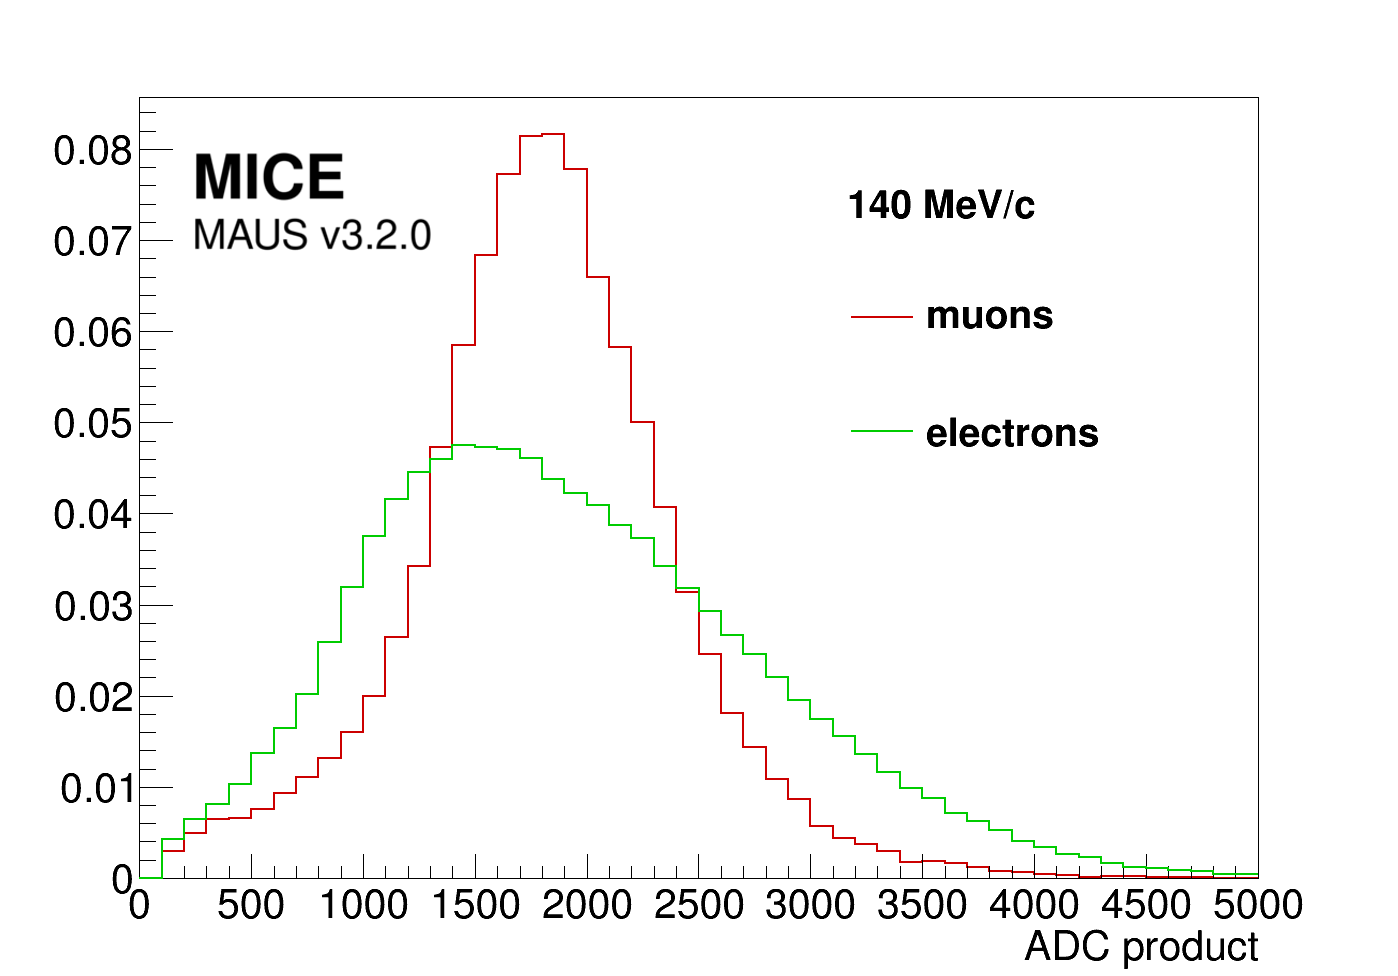
\includegraphics[width=0.49\columnwidth]{./04-KL/Figures/mu_vs_e_140MeV.png}
    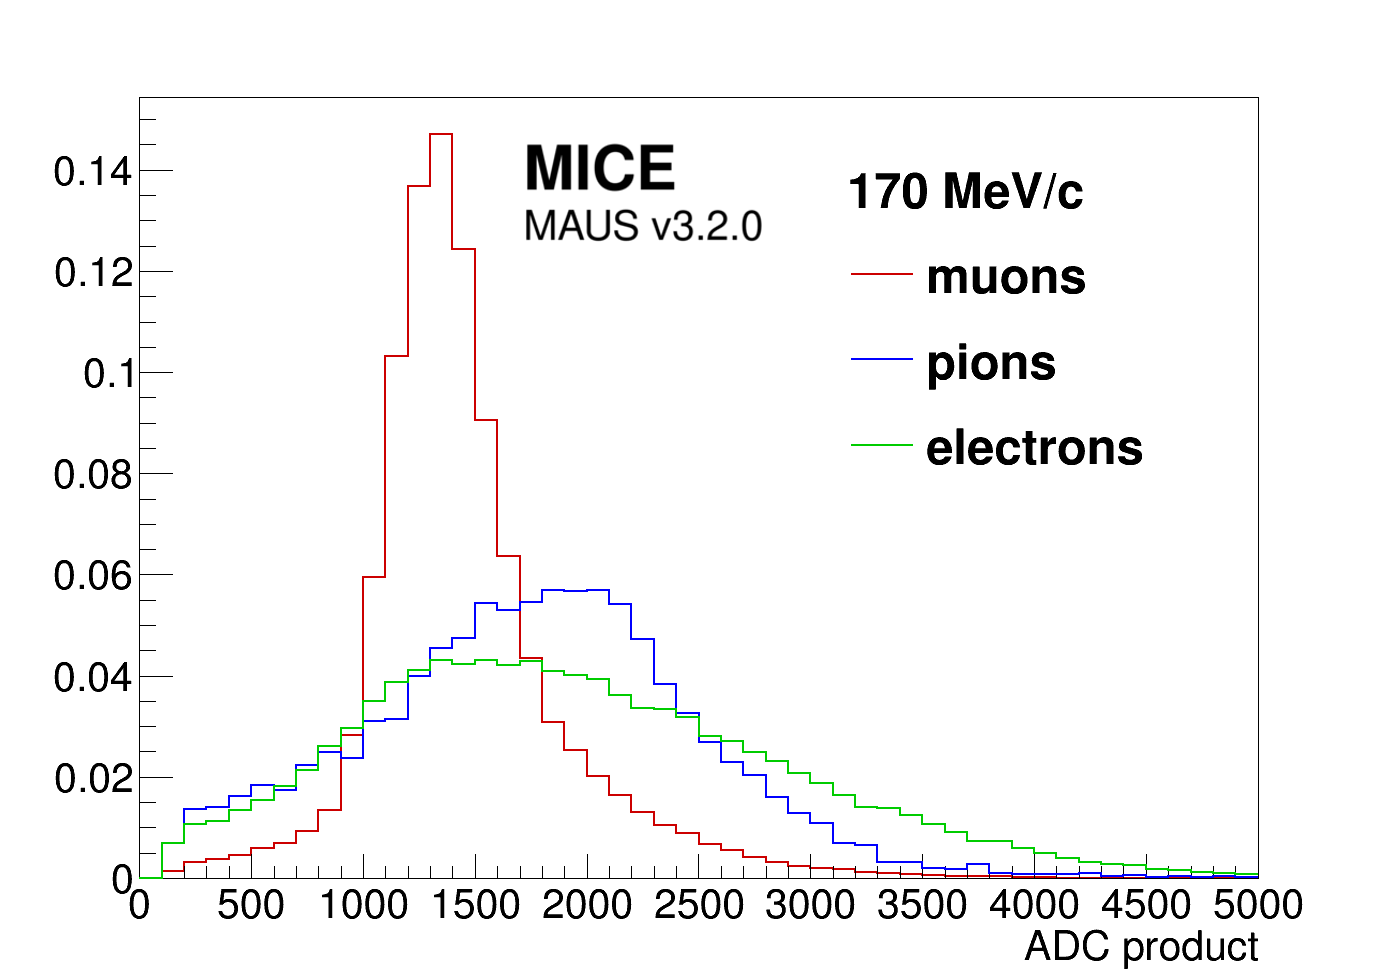
\includegraphics[width=0.49\columnwidth]{./04-KL/Figures/mu_vs_pi_vs_e_170MeV.png} 
    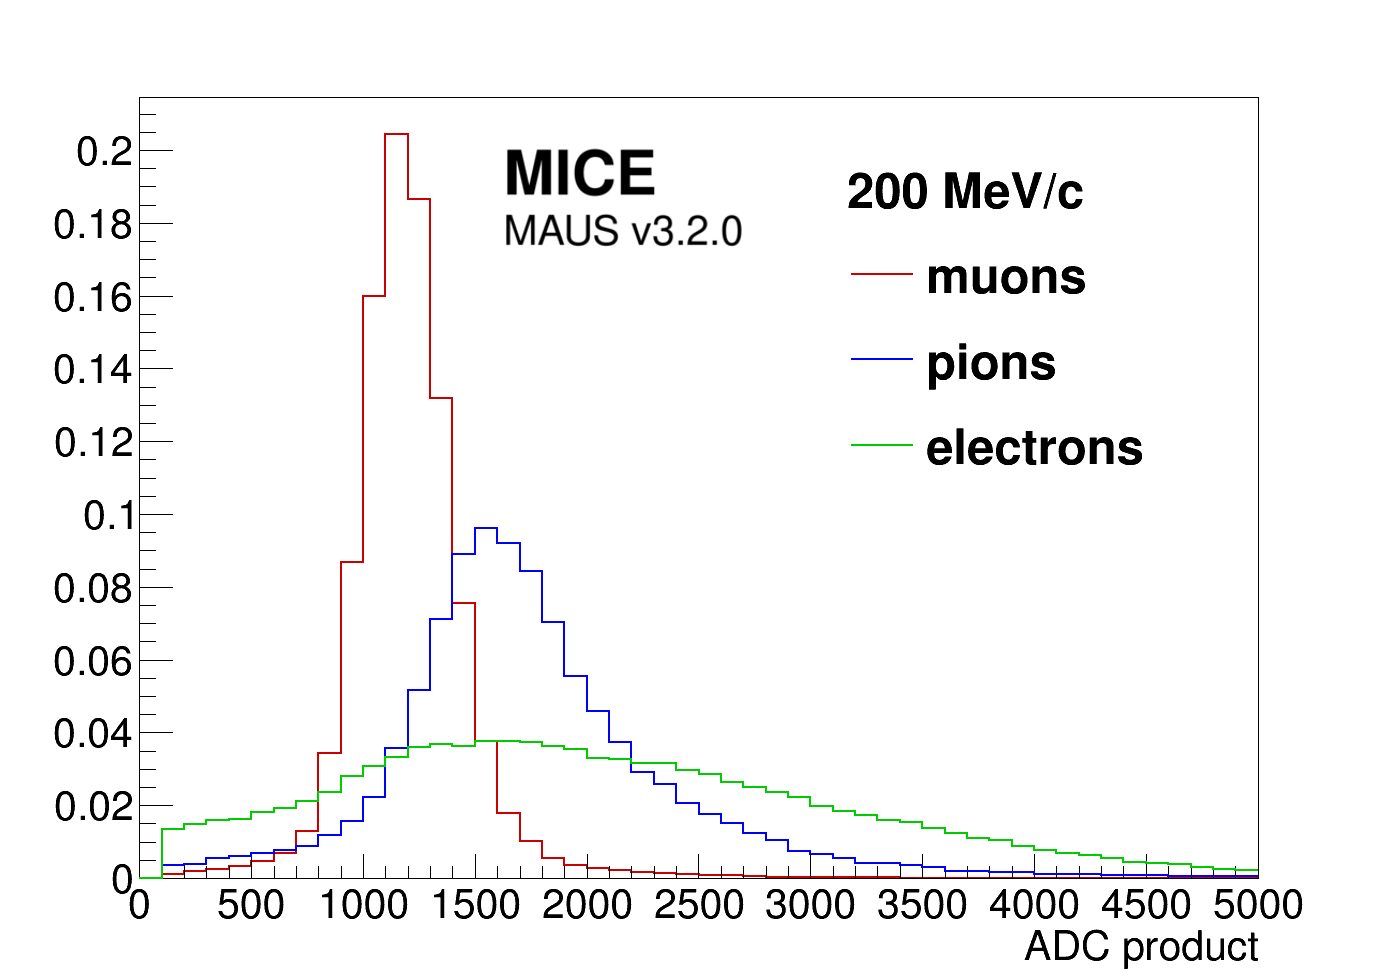
\includegraphics[width=0.49\columnwidth]{./04-KL/Figures/mu_vs_pi_vs_e_200MeV.png}
    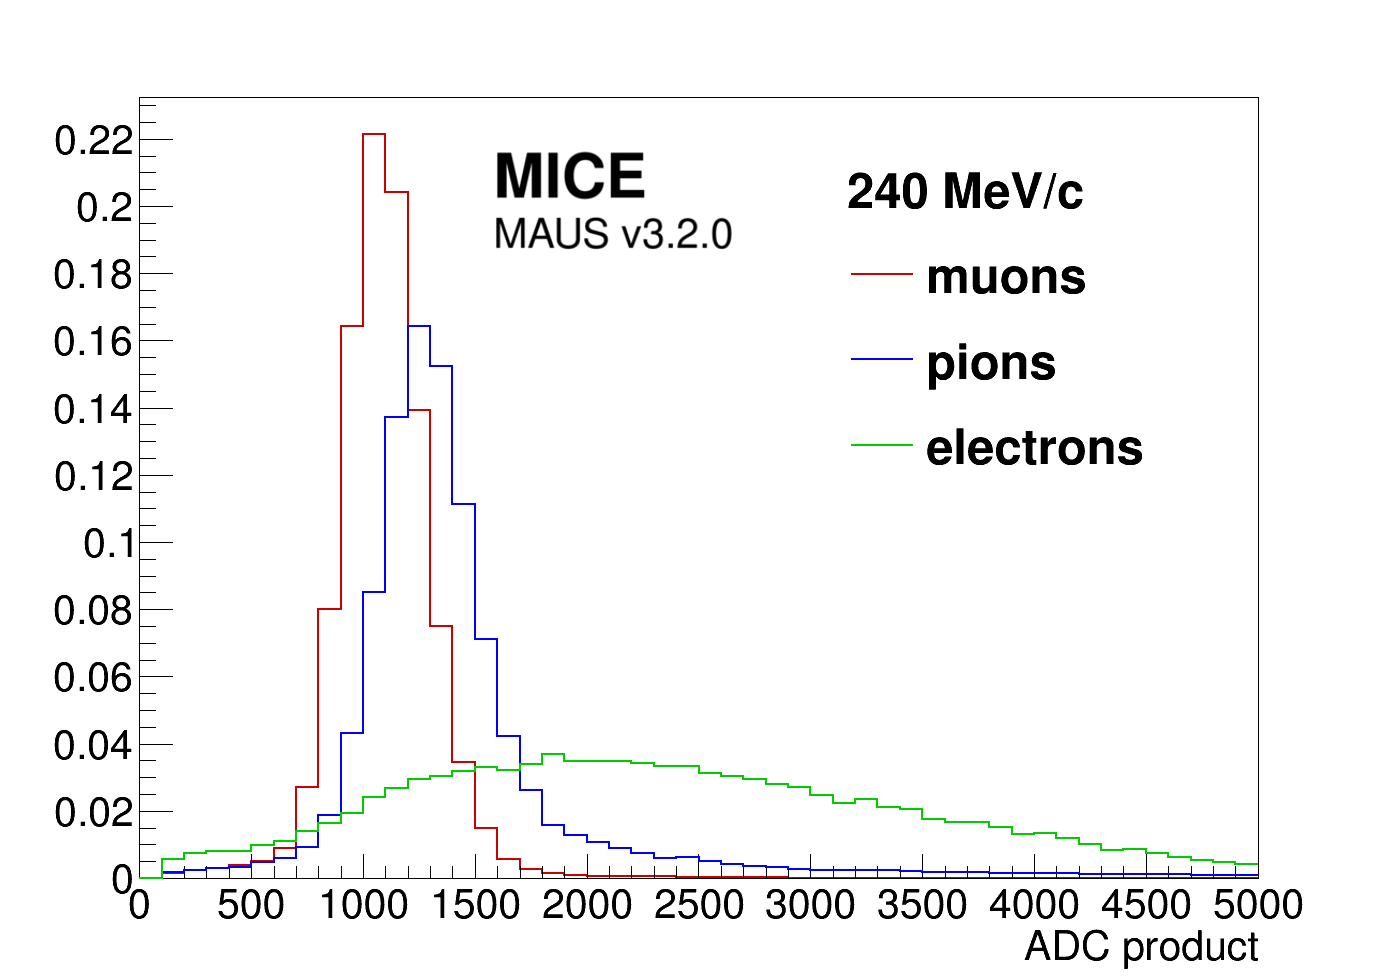
\includegraphics[width=0.49\columnwidth]{./04-KL/Figures/mu_vs_pi_vs_e_240MeV.png}  	
    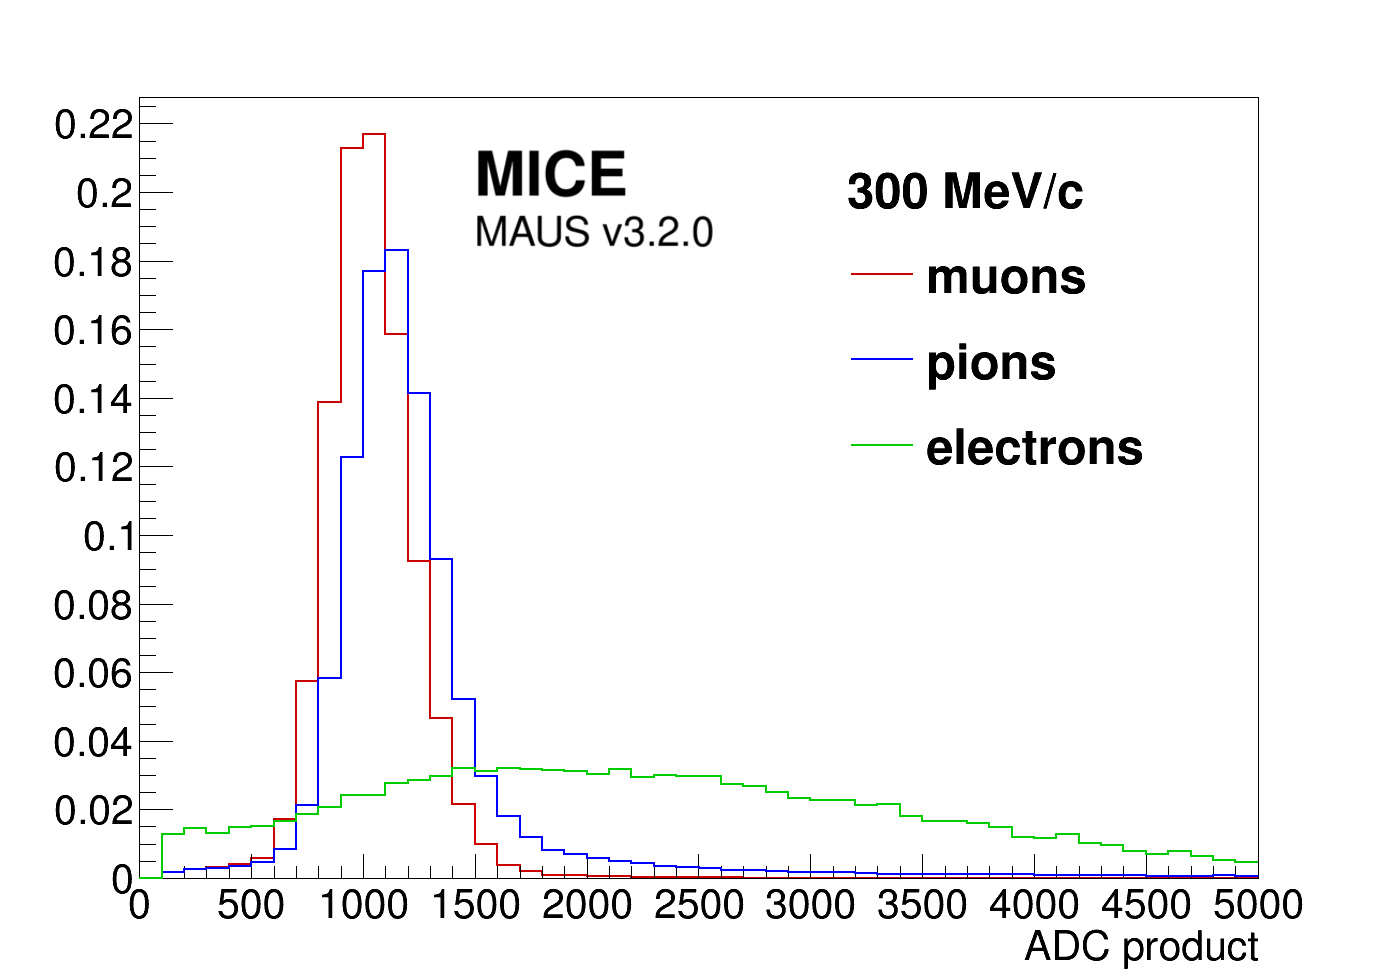
\includegraphics[width=0.49\columnwidth]{./04-KL/Figures/mu_vs_pi_vs_e_300MeV.png}
  \end{center}
  \caption{
    Comparison of ADC products of muons (red), pions (blue) and electrons (green) traversing the KL, at 140
    MeV/$c$ (top left), 170 MeV/$c$ (top right), 200 MeV/$c$ (middle
    left), 240 MeV/$c$ (middle right) and 300 MeV/$c$ (bottom).
  }
  \label{fig:KL4}
\end{figure}
\begin{figure}
  \begin{center}
    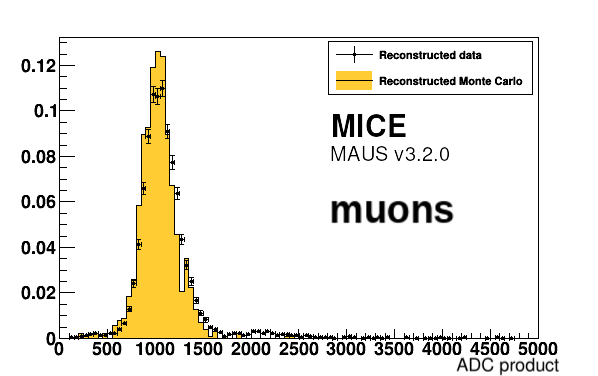
\includegraphics[width=0.49\columnwidth]{./04-KL/Figures/muon_mc_vs_data_edited.png}
    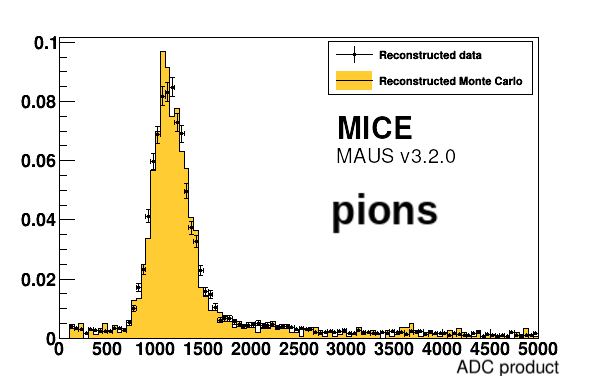
\includegraphics[width=0.49\columnwidth]{./04-KL/Figures/pion_mc_vs_data_edited.png}
  \end{center}
  \caption{
    Comparison between data and Monte Carlo simulation of KL response
    to muons (left) and pions (right) at 300 MeV/$c$.
  } 
  \label{fig:KL_mc_vs_data}
\end{figure}

The ADC~product distribution measured using a 300\,MeV/$c$ beam is
compared to the MAUS simulation of the detector response in
figure~\ref{fig:KL_mc_vs_data}.
The simulation takes into account the light production distribution of the
scintillating fibres, and the response of the PMTs for which the gain was
approximately $2 \times 10^6$. 
The data is well described by the simulation.
